
\documentclass{IOS-Book-Article}

\usepackage{mathptmx}
\usepackage{graphicx}
%\usepackage{times}
%\normalfont
%\usepackage[T1]{fontenc}
%\usepackage[mtplusscr,mtbold]{mathtime}
%
\begin{document}
\begin{frontmatter}              % The preamble begins here.

%\pretitle{Pretitle}
\title{Gated Sensor Fusion: A way to Improve the Precision of Ambulatory Human Body Motion Estimation}
%\runningtitle{IOS Press Style Sample}
%\subtitle{Subtitle}

\author[A]{Alberto Olivares%
\thanks{Corresponding Author: CITIC-UGR, Calle Periodista Rafael Gomez Montero, 2; E-mail:aolivares@ugr.es.}},
\author[A]{J. M. G\'orriz},
\author[A]{J. Ram\'irez}
and
\author[B]{Gonzalo Olivares}


\runningauthor{Alberto Olivares et al.}
\address[A]{Dept. of Signal Processing, Telematics and Communications (TSTC), University of Granada, SPAIN}
\address[B]{Dept. of Computer Architecture and Computer Technology (ATC), University of Granada, SPAIN}

\begin{abstract}
Human body motion is usually variable in terms of intensity and, therefore, any Inertial Measurement Unit attached to a subject will measure both low and high angular rate and accelerations. This can be a problem for the accuracy of orientation estimation algorithms based on adaptive filters such as the Kalman filter, since both the variances of the process noise and the measurement noise are set at the beginning of the algorithm and remain constant during its execution. Setting fixed noise parameters burdens the adaptation capability of the filter if the intensity of the motion changes rapidly. In this work we present a conjoint novel algorithm which uses a motion intensity detector to dynamically vary the noise statistical parameters of different approaches of the Kalman filter. Results show that the precision of the estimated orientation in terms of the RMSE can be improved up to 29\% with respect to the standard fixed-parameters approaches.
\end{abstract}

\begin{keyword}
Human motion\sep Orientation estimation\sep MARG sensors\sep Kalman filtering\sep Intensity detection 
\end{keyword}

\end{frontmatter}

\thispagestyle{empty}
\pagestyle{empty}

\section{Introduction}
\label{sec:introduction}
\indent \indent Measuring human motion is of key importance in medical practice as it provides a way to improve the diagnosis and treatment of several diseases. For instance, it helps physicians to assess patients with neurodegenerative diseases which cause disruptions in the motor system \cite{sprdlik_tremor_2009}, as well as to improve the quality of rehabilitation processes\cite{yaqin_tao_novel_2008}, reduce the risk of falls \cite{howcroft2013}, analyze gait \cite{macwilliams_functional_2010}, study sleep disorders \cite{Tang2004} and detect unnoticed nocturnal epileptic seizures \cite{Poh2012}.

Human motion can be measured in different ways and there are distinct factors that need to be taken into account when selecting an approach to measure it. The reference point from which we want to gather the measurements is one of them. The reference point can be either fixed in space or included in the object. If we choose the former, a possible option is to set a room which has cameras acting as observers which are placed in different fix positions as in \cite{cerveri_robust_2003}. Vicon\textregistered \,cameras \cite{vicon} and Microsoft's Kinect \cite{kinect} are regularly used in camera-based motion analysis systems \cite{chung_validity_2011}. Camera-based systems are very accurate but limit the movements of the patients to a room. On the other hand, if we choose the latter, our system will be able to perform ambulatory measurements. For such an approach, we need a device that is attached to the patient's body and measures its relative acceleration, angular rate and heading. Hence, our system needs from magnetic and inertial sensors, and more specifically, acceleration sensors (accelerometers), angular rate sensors (gyroscopes) and magnetic field sensors (magnetometers). Our work uses the data of a set of devices that can be attached to different parts of human body and compute their positioning angles. Such devices including magnetic and inertial sensors are generally known as Magnetic Inertial Measurement Units (MIMUs).

Data measured by the MIMUs need to be processed to compute the orientation of the body of the patient which is wearing them. Within the last decade, different orientation estimation algorithms have been employed to process the information measured with MIMUs in order to monitor human motion. These algorithms are used to fuse the information coming from all three sensors. The Kalman fiter \cite{Welch2001} is by far the most popular approach to carry out such a sensor fusion. 

Most algorithms, including Kalman filters, have a set of parameters which are constant during the execution and which are critical to their performance. These parameters control the level of confidence which is given to the data coming from one of the sensors which is known as the observation. It is also known that the observation (for orientation estimation), which is usually computed using the measured acceleration, is less accurate when the intensity of motion is intense i.e. the linear acceleration is not negligible with respect to the gravity. Therefore, giving a fixed value to these parameters, when monitoring motion with changing intensity, may decrease the accuracy of the estimation. \\
In this work, we propose a novel strategy to improve the ambulatory estimation of the orientation of human body using magnetic and inertial sensors. Our approach is based on the dynamical modification of some of the formerly fixed parameters of the Kalman filter according to the intensity of the motion. The intensity of the motion is detected using frequency analysis of the acceleration signals. This will improve the adapting ability of the orientation algorithms, and therefore, their performance.\\

The rest of the paper is structured as follows; section \ref{sec:previous_work} includes a revision of the state of the art; next the theoretical background of the intensity detector and the gated sensor fusion is presented in section \ref{sec:theory}; experiments carried out to test the gated sensor fusion approach are shown in section \ref{sec:experiments} and subsequently discussed in section \ref{sec:discussion}; finally, conclusions and future work are drawn in section \ref{sec:conclusions}.

\section{Previous Work}
\label{sec:previous_work}

\subsection{Orientation Estimation Algorithms}
\label{subsec:orientation_review}
\indent \indent Orientation estimation methods started to be developed in the seventies in order to be applied in space missions. Algorithms were developed to determine the orientation of the spaceship with respect to different reference frames.
Examples of these early methods can be found in \cite{lerner78} and \cite{shuster_three-axis_1981} which describe the TRIAD and QUEST methods respectively. The TRIAD algorithm provides a deterministic solution for the attitude based on two vector observations and two vector references (which, in our case, can be the a priori known gravity and local Earth magnetic field vectors) which are used to compute the attitude matrix. The QUEST algorithm minimizes a loss function to find the optimal quaternions representing the attitude. In our context (determination of human body orientation using magnetic and inertial sensors), these methods solely use the accelerometer and the magnetometer. To avoid problems related to high intensity motion, \cite{yun_design_2006} fuses QUEST algorithm with the integration of angular rate using an Extended Kalman Filter (EKF). \\
\indent Many variations of these methods have been proposed during the last decades mainly by Malcolm D. Shuster \cite{malcolmPub1}, F. Landis Markley \cite{Landis2000}, and Xiaoping Yun \cite{marins_extended_2001}. In \cite{marins_extended_2001} a Gauss-Newton iteration algorithm is employed to find the best quaternion which relates the measured accelerations and earth magnetic field in the body frame to calculated values in the earth coordinate frame. Such quaternion is fused afterwards with angular rate using an EKF. This approach provides good results but adds high computational cost due to the minimization procedure which has to be computed for every set of measurements. \\
\indent Examples of algorithms to compute Euler angles without employing quaternions can be found in \cite{Salhuana2012}.\\
\indent A very complete survey of nonlinear orientation estimation methods can be found in \cite{crassidis_survey_2007} and a comparison between some of the most popular orientation filter algorithms is also found in \cite{young_comparison_2009}.

\subsection{Estimation of orientation applied to human body position and motion monitoring}
\label{subsec:orientation_human_body_soa}
\indent \indent As said in the introduction, monitoring of human body motion is one of the most popular fields of application of orientation estimation methods. In this case, instead of computing the orientation of a spaceship, the orientation of different segments of human body is estimated with respect to a fixed frame. The orientation angles are then used to represent the position of the body at every time instant. \\
\indent Zhang et al. propose in \cite{zhang_ambulatory_2009} a Hybrid Dynamic Bayesian Network to model the nonlinear hip angle dynamics and a Gaussian Particle Filter to estimate the hip angle during gait cycles from the measurements of a wearable accelerometer which is attached to the thighs. They achieve a minimum error of $1.50^{\circ}$ RMS in the orientation. However, since the angle estimation is only based on the accelerometer readings this algorithm will likely show larger errors when applied under more intense motion conditions. \\
\indent Luinge et al. present in \cite{luinge_ambulatory_2007} a method that uses constraints in the elbow to measure the orientation of the lower arm with respect to the upper arm. They use an IMU composed of a triaxial accelerometer and a triaxial gyroscope, and apply a least squares filter that estimates the orientation errors in a way that sets the adduction angle to zero. Their algorithm fails to estimate the orientation properly as it shows errors of up to $40^{\circ}$ RMS.\\
\indent Roetenberg et al. describe in \cite{roetenberg_compensation_2005} a complementary Kalman Filter design to estimate the orientation of human body segments by fusing gyroscope, accelerometer and magnetometer signals from MEMS sensors. The filter estimates the gyroscope error bias, the orientation error and the magnetic disturbance error. The average static and dynamic errors are $1.4^{\circ}$ and $2.6^{\circ}$ RMS, respectively.\\
\indent Luinge et al. describe in \cite{luinge_inclination_2004} the design and performance of a Kalman filter to estimate inclination from the signals of a triaxial accelerometer. They achieve an accuracy of $2^{\circ}$ RMS for quasi-static motion. \\
\indent Favre et al. present in \cite{favre_quaternion-based_2006} two methods to fuse a triaxial gyroscope with a triaxial accelerometer to measure rotations. These methods compute the orientation quaternion using the acceleration measurements during quasi-static instants and update it using the rotation quaternion obtained from the angular rate measurements during dynamic instants. \\
\indent Similarly, Sabatini proposes in \cite{sabatini_quaternion-based_2005} an interpolation technique applied to attitude quaternions to improve the accuracy of orientation and positioning estimates. It obtains an accuracy of $14.6^{\circ}$ RMSE during one gait cycle and $14.8^{\circ}$ RMSE during two gait cycles. Additionally, it describes a quaternion based extended Kalman filter (EKF) algorithm that achieves an accuracy close to $4^{\circ}$ RMSE.\\
\indent Favre et al. propose a method based on a leg movement to align two inertial measurement units fixed on the thigh and shank segments. They combine this method with their fusion algorithm \cite{favre_quaternion-based_2006}, to obtain an error within the $[0^{\circ},3.4^{\circ}]$ range for different knee quasi-static movements. They employ an IMU composed of a triaxial accelerometer and a triaxial gyroscope.\\ 
\indent We conclude the review of the state of the art with the work by Amasay et al, who describe in \cite{amasay_validation_2009} a simple method based only on the decomposition of gravity acceleration to estimate the pitch angle. They obtain a RMSE of less than $1^{\circ}$ only during quasi-static conditions. This simple method is absolutely non valid to estimate the orientation of a body moving with medium to high intensity as it does not apply any sensor fusion strategies.

\section{Theoretical Background}
\label{sec:theory}
\indent \indent Our proposal can be divided in two parts; first, an intensity detection algorithm needs to be applied to determine whether patient's motion is smooth or intense; next, a gated Kalman filter sensor fusion algorithm is applied to estimate the orientation from the ga\-the\-red acceleration, angular rate and magnetic field, using the optimal parameter values according to the sensed intensity level. 

\subsection{Intensity Detectors}
\label{subsec:intensity_detectors}
\indent \indent There are many different algorithms which can be used to determine the intensity of motion. Most of them are based on the time analysis of the magnitude of acceleration and/or angular rate. In \cite{olivares_detection_2012} it was demonstrated that methods based on the frequency analysis of these magnitudes have larger precision to classify between smooth and intense motion. More specifically, the Framed Spectrum Detector (FSD) and the Long Term Spectral Envelope Detector (LTSED) offered accuracy rates up to 98\%. In this work, we have employed the FSD detector due to its lower computational complexity and high precision.  

The output of the FSD is compared with a predefined threshold to obtain a binary marker which indicates the detected intensity ('0' for smooth motion and '1' for intense motion). Therefore, this marker is also used to change the value of the parameters of the orientation estimation algorithms to adequate them in real time to the sensed intensity. 

For this work, we used the magnitude of the measured acceleration as the input to the FSD, and the output of the FSD can be computed applying the following expression,
\begin{equation}
\mbox{V}(\mathbf{n})=10\log_{10}\left(\frac{1}{\mbox{N}_{\scriptsize \mbox{FFT}}}\sum_{l=0}^{\mbox{N}_{\scriptsize \mbox{FFT}}-1}\frac{\mbox{X}^{2}(l,n)}{\mbox{N}^{2}(l)}\right)<\gamma
\label{eq:fsd}
\end{equation}
where $\mbox{N}_{\scriptsize \mbox{FFT}}$ is the resolution of the Fast Fourier Transform, N($l$) is the average noise spectrum magnitude for the $l$ band, $\mbox{X}(l,n)$ is the spectrum of the input signal for the  $l$ band at frame $n$ and $\gamma$ is an empirical predefined threshold. 

Figure \ref{fig:FSD_output} shows the output of the FSD detector and the estimated activity marker superposed to the reference pitch angle (rotation angle around Y axis). Intense motion periods can be easily seen due to the higher rate of change in the orientation angle. 
\begin{figure}[t]
\centering
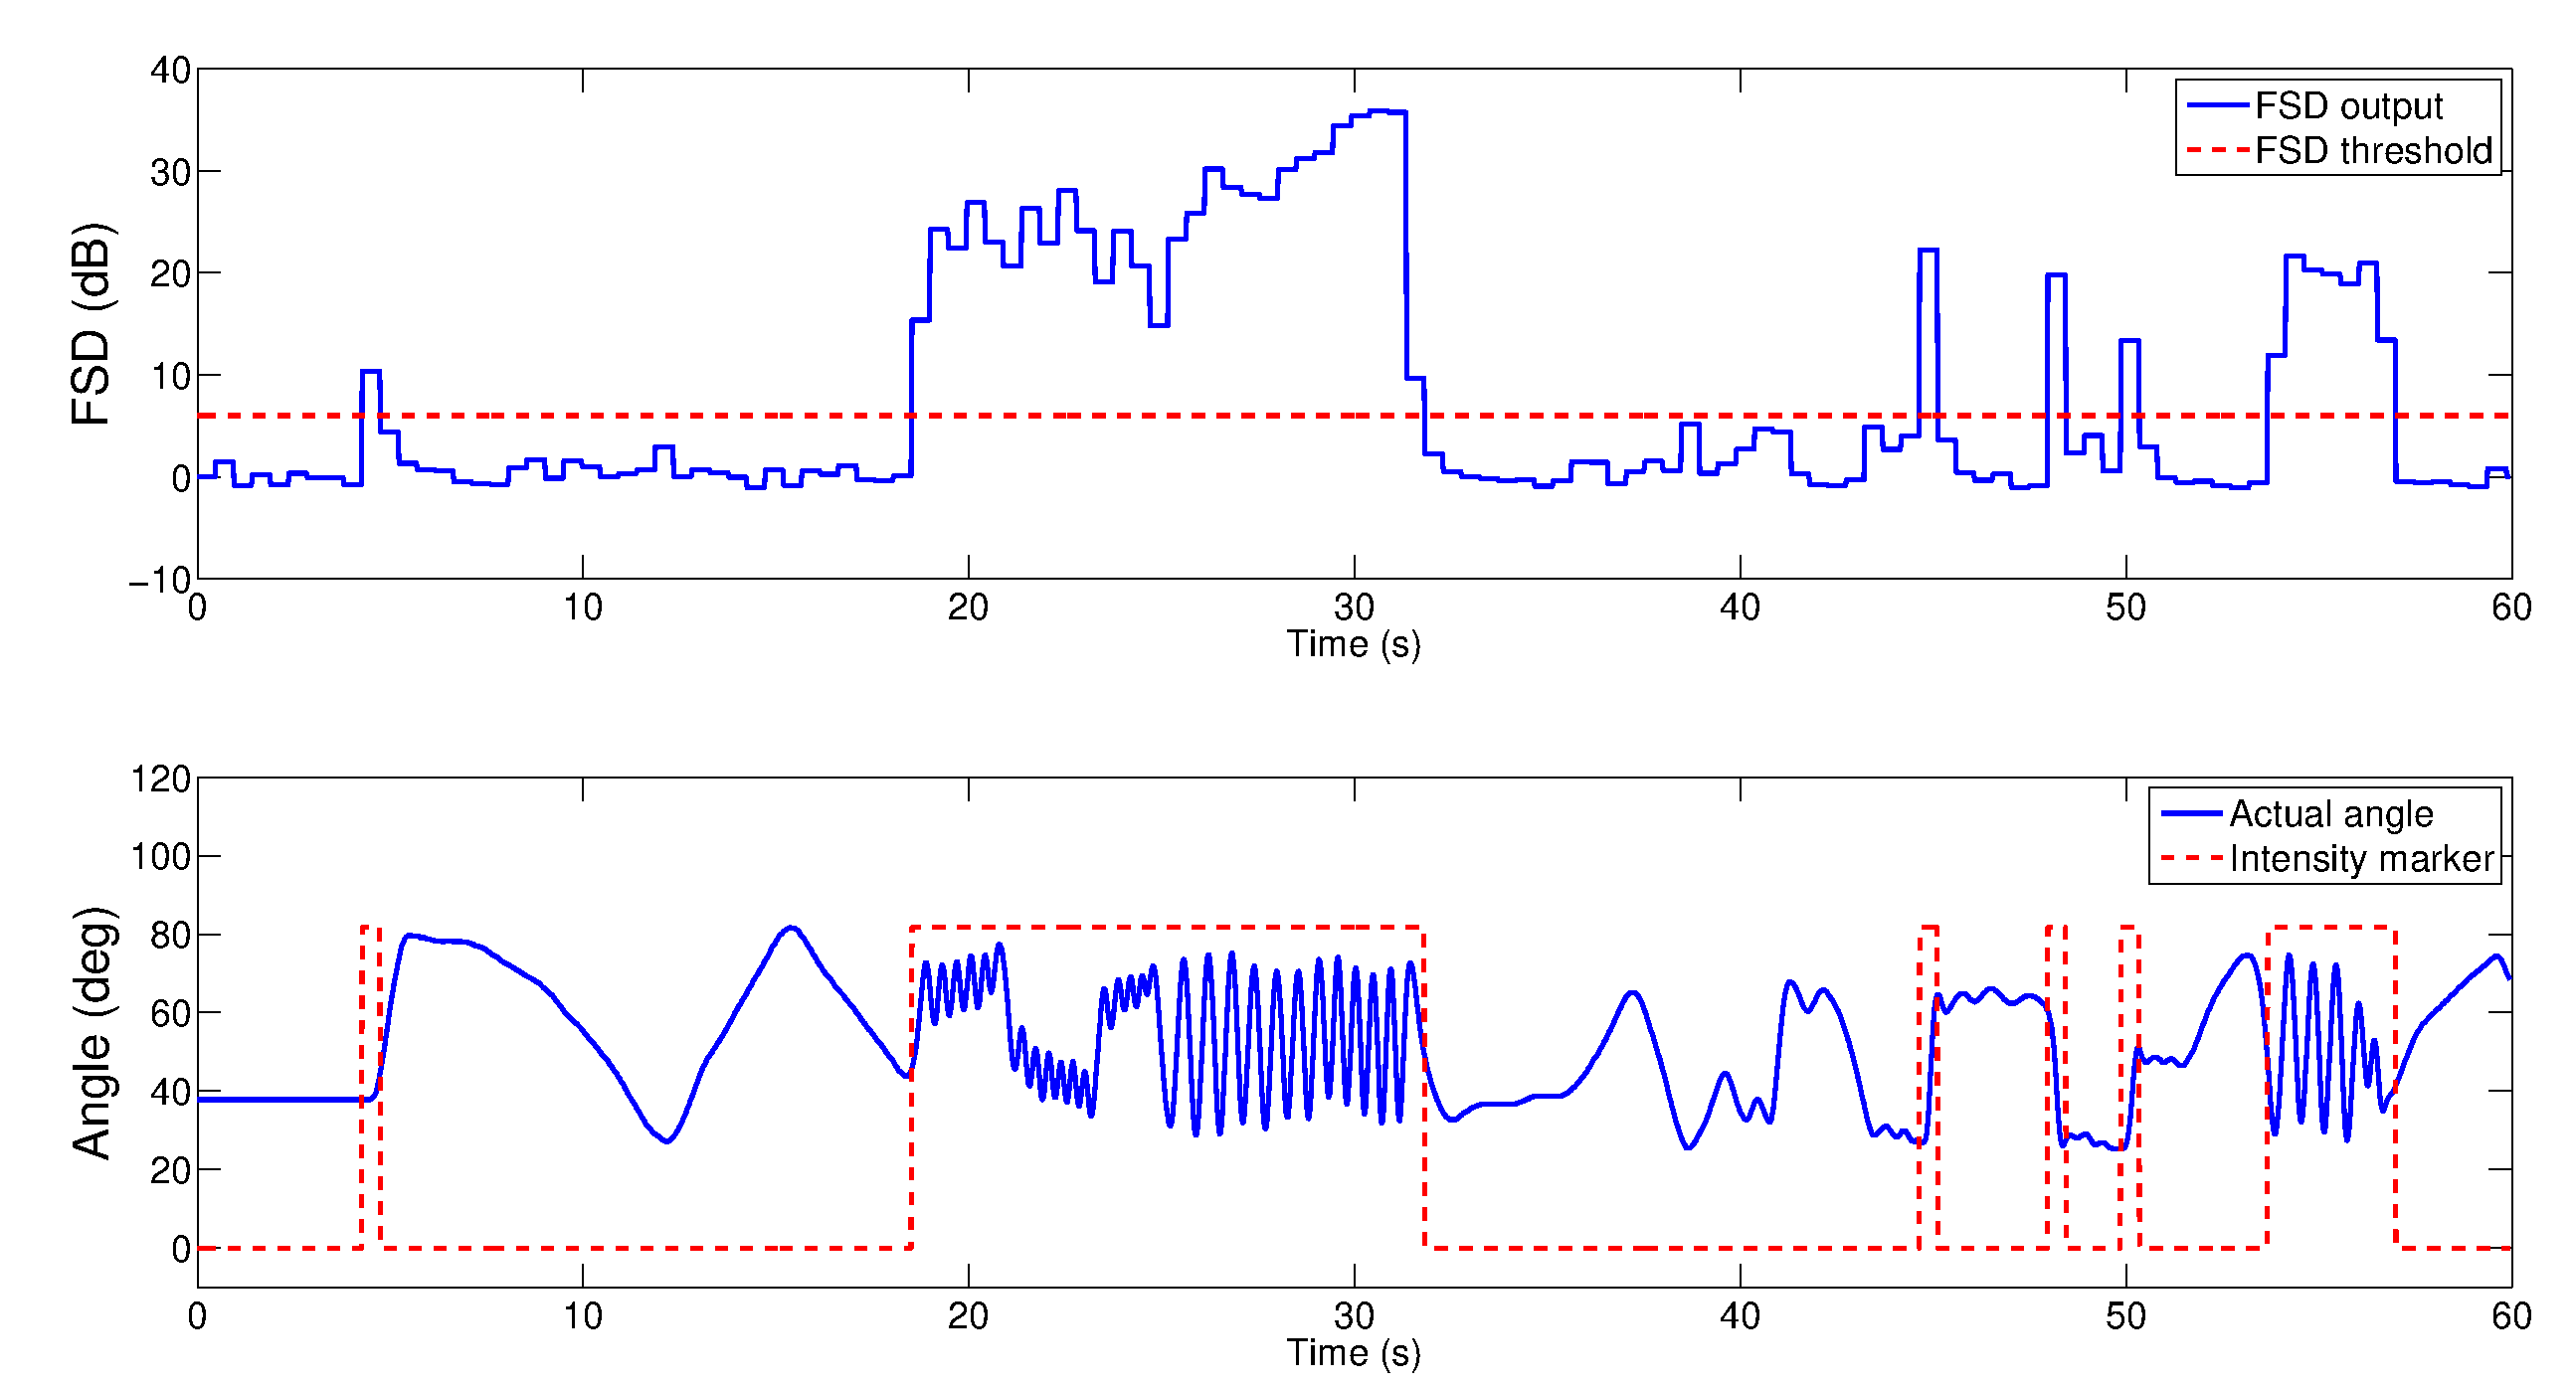
\includegraphics[width=1\textwidth]{figures/FSD_output.eps}
\caption{Output of the framed spectrum detector (top). Reference angle vs. intensity marker (bottom).}
\label{fig:FSD_output}
\end{figure}

\subsection{Gated Orientation Estimation Algorithms}
\label{subsec:gated_algorithms}
\indent \indent As said in the introduction and in section \ref{subsec:orientation_review}, most orientation estimation algorithms are based on the Kalman filter. The Kalman filter is used to fuse the data ga\-the\-red by all the sensors (accelerometer, gyroscope and magnetometer). This fusion is strictly necessary since none of the sensors can offer accurate orientation estimates when used individually. Some of the well known problems of the individual use of the sensors to estimate the orientation are:
\begin{itemize}
\item \textit{Accelerometer}: Orientation estimates can be obtained from the acceleration readings by decomposing the Earth's gravity vector. However, this approach is only valid when the measured linear acceleration is negligible with respect to the gravity acceleration. That is, the orientation estimates are only valid if the subject's motion is very smooth.
\item \textit{Gyroscope}: Orientation estimates can be obtained from the gyroscope by integrating the gathered angular rate. This approach suffers from the devastating effects of the integration of the noise present in the sensor's output. The integration of the noise causes a large time-increasing drift which introduces large errors in a few seconds time.
\item \textit{Magnetometer}: Orientation estimates can be obtained from the magnetic field readings by decomposing the Earth's magnetic field vector. This approach is only valid in magnetically clean environments since large disruptions can be produced by externally induced magnetic fields. Since this kind of completely clean environments is rare nowadays, the magnetometer orientation estimates are rather inaccurate. However, magnetometers are necessary if the heading angle (rotation around Z axis) is needed.
\end{itemize}

\indent Human body motion is usually variable in terms of intensity. We move with both smooth and intense movements and, therefore, a MIMU attached to our body will measure both low and high angular rate and accelerations. This can be a problem for the accuracy of the classic Kalman Filter approach since both the variances of the process noise and the measurement noise are set at the beginning of the algorithm and remain constant during its execution. If we consider the linear acceleration as one of the elements of the noise disrupting both the process and the measurement, then, it is straightforward to see that smooth motion will introduce low linear acceleration in the measurements, and therefore, low noise. On the other hand, intense motion is originated by large linear accelerations, so the acceleration readings will be corrupted with these disrupting accelerations which are modeled as noise. \\
\indent Thus, if we set low process and measurement noises, we are telling the filter that the gravity acceleration prevails the linear acceleration and then, it will rely more on the acceleration readings to estimate the orientation. This can be a problem if the intensity of the motion starts to be changing (which, as we have said, is the usual behavior of human motion) as the adaptation of the filter is burdened by the unchanging process and measurement variances \cite{olivares_thesis}. \\
\indent We thought that the general performance of the classic Kalman Filter could be improved by dynamically changing both process and measurement variances according to the intensity of the motion. To do so, we first set a motion intensity detector to distinguish between low and high intensity. Then, we set the value of the measurement and process noise between two predefined values according to the value of the intensity indicator. Therefore by setting low measurement and process noises when the subject is moving smoothly and setting high values when it is moving intensely, we improve the adapting capability of the filter, and consequently, the precision of the orientation estimation. Figure \ref{fig:GKFDiagram} shows the general diagram of the proposed Gated Kalman Filter architecture.

\begin{figure}[t]
\centering
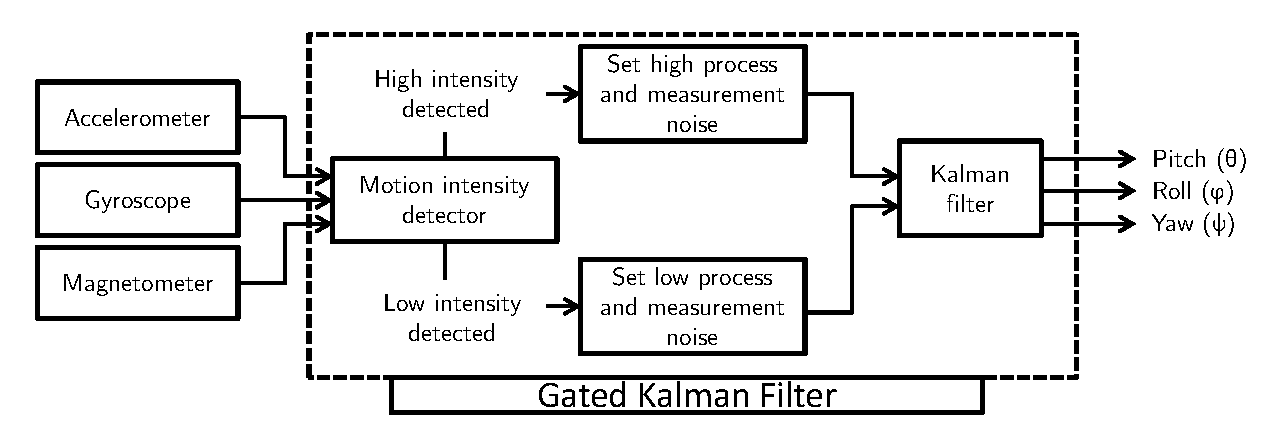
\includegraphics[width=1\textwidth]{figures/GKFDiagram.eps}
\caption{General diagram of the proposed gated sensor fusion approach.}
\label{fig:GKFDiagram}
\end{figure}

\section{Experiments}
\label{sec:experiments}
\indent \indent In order to check the validity of the proposed approach, we carried out a series of experiments. A set of 16 datasets of inertial and magnetic signals (3D acceleration, 3D angular rate and 3D magnetic field) were gathered using a Wagyromag \cite{olivares_wagyromag_2011} MIMU attached to a mechanical device which provides the orientation angle which is used as the ground truth. Each dataset contains data from both smooth and very intense random motions. Each dataset was fed to four different orientation algorithms; two different Kalman Filter (KF) approaches, one using gravity decomposition as the observation and another one using the QUEST algorithm to compute the observation and two different Extended Kalman Filters (EKF) also based on gravity decomposition and the QUEST algorithm. 

As said in the previous section, the parameters to be dynamically varied were the variance of the process noise and the variance of the observation noise which are the main tunning parameters of both the KF and the EKF. These variances are used to populate the process noise and measurement noise covariance matrices, usually denoted as P and R respectively.

The value of both variances was optimized by minimizing the RMSE with respect to the reference, as shown in equation (\ref{eq:rmse}), using the Adaptive Nelder-Mead Simplex Algorithm \cite{gao2012}. The optimal RMSE values were averaged for all 16 datasets and for all methods using a Monte Carlo procedure. Results are shown in table 1 and figure \ref{fig:angles} depicts the reference angle signal vs. two angle estimates, one which uses the regular Kalman Filter and another one using the Gated Kalman Filter. Notice how the adaptability of the gated estimate is larger and how the estimates are closer to the actual value for both smooth and intense motion.

\begin{equation}
RMSE=\sqrt{\frac{1}{N}\sum_{i=1}^{N}\left(angle_{ref}-angle_{estimated}\right)^{2}}
\label{eq:rmse}
\end{equation}

\begin{table}[t]
\centering
\caption{RMSE of estimated pitch angle with respect to the ground truth. Non-gated vs. gated algorithms. Last row shows the percentage of improvement of using the gated approach.}
\label{tab:results}
\footnotesize
\begin{tabular}{ | c | c | c | c | c |}
\hline
					&	KF				&	KF (QUEST)		&	EKF				& 	EKF (QUEST) 	\\\hline
RMSE (deg)			&	$3.00\pm0.72$	&	$1.50\pm0.22$	&	$3.07\pm1.13$	&	$2.26\pm0.48$	\\\hline
					&	G-KF			&	G-KF (QUEST)	&	G-EKF			& 	G-EKF (QUEST) 	\\\hline
RMSE (deg)			&	$2.09\pm0.56$	&	$1.48\pm1.88$	&	$2.35\pm0.97$	&	$2.24\pm0.47$	\\\hline
Improvement (\%) 	&	$29.34\pm12.03$ &   $0.89\pm5.19$	&	$23.31\pm10.70$&	$0.93\pm1.77$	\\
\hline
\end{tabular}
\end{table}

\begin{figure}[t]
\centering
\includegraphics[width=0.9\textwidth]{figures/angles.eps}
\caption{Reference pitch angle vs. angles estimated using both gated and non gated fusion. Smooth motion (up), intense motion (bottom).}
\label{fig:angles}
\end{figure}

\section{Discussion of Results}
\label{sec:discussion}
\indent All four tested methods showed an improvement in the precision of the estimates of the orientation angles when using the gated algorithms. In the case of the standard Kalman Filter and the Extended Kalman Filter, the improvement of the gated approach is remarkable ($29.34\pm12.03$ and $23.31\pm10.70$ respectively). For the KF and the EKF based on the QUEST algorithm the improvement was not as high since QUEST is already similar to a gated algorithm and, therefore, adding a gated fusion architecture has lower impact. 

The effects of the gated approach can be better understood by checking the equations of the standard Kalman Filter.

\begin{itemize}
\item Prediction equations:
\end{itemize}

\begin{equation}
\mathbf{\hat{x}}_{k}^{-}=\Phi\mathbf{\hat{x}}_{k-1}
\label{eq:Kal_fus_pred1}
\end{equation}
\begin{equation}
\mbox{P}_{k}^{-}=\Phi\mbox{P}_{k-1}\Phi^{T}+\mbox{Q}
\label{eq:Kal_fus_pred2}
\end{equation}

\begin{itemize}
\item Update equations:
\end{itemize}

\begin{equation}
\mbox{K}_{k}=\frac{\mbox{P}_{k}^{-}\mbox{H}^{T}}{\mbox{H}\mbox{P}_{k}^{-}\mbox{H}^{T}+\mbox{R}}
\label{eq:Kalman_gain_update_phase}
\end{equation}
\begin{equation}
\mathbf{\hat{x}}_{k}=\mathbf{\hat{x}}_{k}^{-}+\mbox{K}_{k}(\mbox{z}_{k}-\mbox{H}\mathbf{\hat{x}}_{k}^{-})
\label{eq:state_vector_update_phase}
\end{equation}
\begin{equation}
\mbox{P}_{k}=(\mbox{I}-\mbox{K}_{k}\mbox{H})\mbox{P}_{k}^{-}
\label{eq:covariance_matrix_update_phase}
\end{equation}
where $\Phi$ is the state transition matrix, $\mathbf{\hat{x}}_{k}^{-}$ is the a priori state estimate, $\mbox{P}_{k}^{-}$ is the a priori system covariance matrix, $\mbox{Q}$ is the process noise covariance matrix, R is the observation noise covariance matrix, $\mbox{K}_{k}$ is the Kalman filter gain, $\mathbf{\hat{x}}_{k}$ is the a posteriori state estimate and $\mbox{P}_{k}$ is the a posteriori system covariance matrix.

The change in the value of the covariance matrices has shown to be effective to increase the adaptability of the filter under different conditions of motion intensity. As it can be seen in equation (\ref{eq:Kalman_gain_update_phase}), during intense motion periods if we set a large value for the observation noise covariance matrix and a low value for the process noise covariance matrix we decrease the value of the Kalman gain since it is inversely proportional to the former and directly proportional to the latter. The Kalman gain is the core of the adaptation process since it controls the weight which is given to the observation as it is shown in equation (\ref{eq:state_vector_update_phase}). This will make the filter to trust less the estimates computed using the acceleration and therefore, increase the overall precision. On the other hand, during smooth motion periods, the value of the observation noise covariance matrix can be reduced and the filter will give more weight to the estimates coming from the accelerometer data.

The improvement of the precision of the estimates is more evident during periods of intense motion as it can be seen in figure \ref{fig:angles}. This agrees with the expected behavior as the estimates during smooth motion are always more accurate as the observation is closer to the actual orientation value. 

\section{Conclusions and Future Work}
\label{sec:conclusions}
\indent \indent We have presented a novel approach to improve the precision of the orientation of human body motion using magnetic and inertial sensors. The approach is based on applying a gating strategy to Kalman filters to perform sensor fusion. The gating strategy consists on varying the value of the filter's tunning parameters according to the level of sensed motion intensity. To do so, we have developed an intensity detector based on frequency analysis of the gathered acceleration signals which distinguishes between smooth and intense motion. \\
\indent Experiments carried out show an improvement of up to 29\% over the already existing non-gated filters. \\
\indent Our algorithm can be used to monitor the motion and orientation of human body in an ambulatory, which is very important for many medical applications.\\
\indent Future work will be oriented to implement a fuzzy multi-level variation of the parameters of the filter to avoid sharp variations of their value in the transition from smooth to intense motion periods.

\section*{Acknowledgements}
This work was partly supported by the MICINN under the TEC2012-34306 project and the Consejer\'ia de Innovaci\'on, Ciencia y Empresa (Junta de Andaluc\'ia, Spain) under the Excellence Projects P09-TIC-4530 and P11-TIC-7103.

\begin{thebibliography}{99}


\bibitem{sprdlik_tremor_2009}
O.~Sprdlik, Z.~Hurak, M.~Hoskovcova, and E.~Ruzicka.
\newblock Tremor analysis by decomposition of acceleration into gravity and
  inertial acceleration using inertial measurement unit.
\newblock In {\em 9th International Conference on Information Technology and
  Applications in Biomedicine, 2009. {ITAB} 2009}, pages 1--4. {IEEE}, November
  2009.
 
\bibitem{yaqin_tao_novel_2008} 
Yaqin Tao and Huosheng Hu.
\newblock A novel sensing and data fusion system for 3-d arm motion tracking in
  telerehabilitation.
\newblock {\em {IEEE} Transactions on Instrumentation and Measurement},
  57(5):1029--1040, May 2008.

\bibitem{howcroft2013}
Howcroft J., Kofman J. and Lemaire E.D.
\newblock Review of fall risk assessment in geriatric populations using inertial sensors.
\newblock {\em Journal of Neuroengineering and Rehabilitation}, 10(1):91. doi: 10.1186/1743-0003-10-91, 2013.

\bibitem{macwilliams_functional_2010}
{BA} {MacWilliams}, {MC} Sardelli, and {RZ} Tashjian.
\newblock A functional axis based upper extremity model and associated
  calibration procedures.
\newblock {\em Gait \& posture}, 31(2):289--291, February 2010.

\bibitem{Tang2004}
Nicole~K.Y Tang and Allison~G Harvey.
\newblock Correcting distorted perception of sleep in insomnia: a novel
  behavioural experiment?
\newblock {\em Behaviour Research and Therapy}, 42(1):27 -- 39, 2004.

\bibitem{Poh2012}
Ming-Zher Poh, Tobias Loddenkemper, Claus Reinsberger, Nicholas~C. Swenson,
  Shubhi Goyal, Mangwe~C. Sabtala, Joseph~R. Madsen, and Rosalind~W. Picard.
\newblock Convulsive seizure detection using a wrist-worn electrodermal
  activity and accelerometry biosensor.
\newblock {\em Epilepsia}, 53(5):e93--e97, 2012.

\bibitem{cerveri_robust_2003}
P.~Cerveri, A.~Pedotti, and G.~Ferrigno.
\newblock Robust recovery of human motion from video using kalman filters and
  virtual humans.
\newblock {\em Human Movement Science}, 22(3):377--404, August 2003.

\bibitem{vicon}
Motion capture systems from vicon.
\newblock http://www.vicon.com/.
\newblock [Accessed January 14th, 2013].

\bibitem{kinect}
Kinect for {XBOX} 360.
\newblock http://www.xbox.com/kinect.
\newblock [Accessed January 14th, 2013].

\bibitem{chung_validity_2011}
{W.M.} Chung, S.~Yeung, {W.W.} Chan, and R.~Lee.
\newblock Validity of {VICON} motion analysis system for upper limb kinematic
  measurement - a comparison study with inertial tracking xsens system.
\newblock {\em Hong Kong Physiotherapy Journal}, 29(2):97, December 2011.

\bibitem{Welch2001}
G.~Welch and G.~Bishop.
\newblock An introduction to the kalman filter.
\newblock {\em Notes of ACM SIGGRAPH tutorial on the Kalman filter}, 2001.

\bibitem{lerner78}
Gerald~M. Lerner.
\newblock {\em "Three-Axis Attitude Determination" in Spacecraft Attitude
  Determination and Control}.
\newblock Springer Scientific + Business Media, 1978.

\bibitem{shuster_three-axis_1981}
M~D Shuster and S.~D. Oh.
\newblock Three-axis attitude determination from vector observations.
\newblock {\em Journal of Guidance Control and Dynamics}, 4(1):70--77, 1981.

\bibitem{yun_design_2006}
Xiaoping Yun and {E.R.} Bachmann.
\newblock Design, implementation, and experimental results of a
  quaternion-based kalman filter for human body motion tracking.
\newblock {\em Robotics, {IEEE} Transactions on}, 22(6):1216 --1227, December
  2006.

\bibitem{malcolmPub1}
Malcolm d. shuster. publications 2000-present.
\newblock {http://goo.gl/lhePZ}.
\newblock [Accessed January 14th, 2013].

\bibitem{Landis2000}
Francis~Landis Markley and Daniele Mortari.
\newblock {Quaternion Attitude Estimation using Vector Observations}.
\newblock {\em The Journal of the Astronautical Sciences}.

\bibitem{marins_extended_2001}
{J.L.} Marins, Xiaoping Yun, {E.R.} Bachmann, {R.B.} {McGhee}, and {M.J.} Zyda.
\newblock An extended kalman filter for quaternion-based orientation estimation
  using {MARG} sensors.
\newblock In {\em 2001 {IEEE/RSJ} International Conference on Intelligent
  Robots and Systems, 2001. Proceedings}, volume~4, pages 2003 --2011 vol.4,
  2001.

\bibitem{Salhuana2012}
Tilt sensing using linear accelerometers (freescale semiconductor application
  note).
\newblock http://goo.gl/0duLQ.
\newblock [Accessed January 14th, 2013].

\bibitem{crassidis_survey_2007}
John~L. Crassidis, F.~Landis Markley, and Yang Cheng.
\newblock A survey of nonlinear attitude estimation methods.
\newblock {\em Journal of Guidance, Control, and Dynamics}, 30(1):12--28,
  January 2007.

\bibitem{young_comparison_2009}
A.~D. Young.
\newblock Comparison of orientation filter algorithms for realtime wireless
  inertial posture tracking.
\newblock In {\em Wearable and Implantable Body Sensor Networks, International
  Workshop on}, volume~0, pages 59--64, Los Alamitos, {CA}, {USA}, 2009. {IEEE}
  Computer Society.

\bibitem{zhang_ambulatory_2009}
Zhiqiang Zhang, Zhipei Huang, and Jiankang Wu.
\newblock Ambulatory hip angle estimation using gaussian particle filter.
\newblock {\em Journal of Signal Processing Systems}, 58(3):341--357, June
  2009.

\bibitem{luinge_ambulatory_2007}
{H.J.} Luinge, {P.H.} Veltink, and {C.T.M.} Baten.
\newblock Ambulatory measurement of arm orientation.
\newblock {\em Journal of Biomechanics}, 40(1):78--85, 2007.

\bibitem{roetenberg_compensation_2005}
D.~Roetenberg, {H.J.} Luinge, {C.T.M.} Baten, and {P.H.} Veltink.
\newblock Compensation of magnetic disturbances improves inertial and magnetic
  sensing of human body segment orientation.
\newblock {\em {IEEE} Transactions on Neural Systems and Rehabilitation
  Engineering}, 13(3):395--405, September 2005.

\bibitem{luinge_inclination_2004}
H.~J Luinge and P.~H Veltink.
\newblock Inclination measurement of human movement using a {3-D} accelerometer
  with autocalibration.
\newblock {\em {IEEE} Transactions on Neural Systems and Rehabilitation
  Engineering}, 12(1):112--121, March 2004.

\bibitem{favre_quaternion-based_2006}
J.~Favre, {B.M.} Jolles, O.~Siegrist, and K.~Aminian.
\newblock Quaternion-based fusion of gyroscopes and accelerometers to improve
  {3D} angle measurement.
\newblock {\em Electronics Letters}, 42(11):612 -- 614, May 2006.

\bibitem{sabatini_quaternion-based_2005}
A.~M. Sabatini.
\newblock Quaternion-based strap-down integration method for applications of
  inertial sensing to gait analysis.
\newblock {\em Medical \& Biological Engineering \& Computing}, 43(1):94--101,
  February 2005.

\bibitem{amasay_validation_2009}
Tal Amasay, Keely Zodrow, Laurel Kincl, Jennifer Hess, and Andrew Karduna.
\newblock Validation of tri-axial accelerometer for the calculation of
  elevation angles.
\newblock {\em International Journal of Industrial Ergonomics}, 39(5):783--789,
  September 2009.
\newblock [Accessed January 14th, 2013].

\bibitem{olivares_detection_2012}
Alberto Olivares, Javier Ramírez, Juan~M. Górriz, Gonzalo Olivares, and Miguel
  Damas.
\newblock Detection of (in)activity periods in human body motion using inertial
  sensors: A comparative study.
\newblock {\em Sensors}, 12(5):5791--5814, May 2012.

\bibitem{olivares_thesis}
Alberto Olivares Vicente,
\newblock Signal Processing of Magnetic and Inertial Sensor's Signals applied to Human Body Motion Monitoring. 
\newblock{\em PhD Thesis dissertation.}
\newblock University of Granada, Spain, April 2013.

\bibitem{olivares_wagyromag_2011}
A.~Olivares, G.~Olivares, F.~Mula, {J.M.} Gorriz, and J.~Ramirez.
\newblock Wagyromag: Wireless sensor network for monitoring and processing
  human body movement in healthcare applications.
\newblock {\em Journal of Systems Architecture}, 57(10):905--915, nov 2011.

\bibitem{gao2012}
Fuchang Gao, Lixing Han. 
\newblock Implementing the Nelder-Mead simplex algorithm with adaptive parameters
\newblock {\em Computational Optimization and Applications}, January 2012, Volume 51, Issue 1, pp 259-277.

\end{thebibliography}
\end{document}
